I en ikke-inverterende forsterker er \emph{ikke} signalet faseforskjøvet 90°,
som i en inverterende forsterker.

\begin{figure}[H]
  \caption{Ikke-inverterende forsterker}
  \centering
  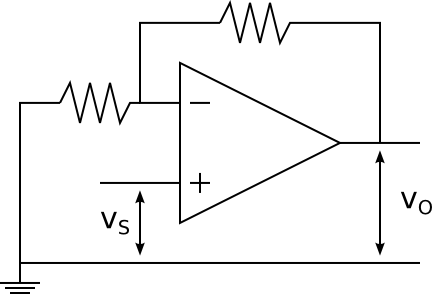
\includegraphics[width=0.5\textwidth]{./img/ikkeinv}
\end{figure}

$$v_O = \frac{R_1+R_2}{R_2} \cdot v_S
= \left( \frac{R_1}{R_2} + 1 \right) \cdot v_S$$

$$A_{vf} = \frac{v_O}{v_S} = \frac{R_1}{R_2}+1$$



\paragraph{Spenningsfølger} \mbox{} \\
Hvis $R_1$ eller $R_2$ er null blir forsterkningen 1.
Dette kalles en spenningsfølger.
Utgangen kan drive mer strøm enn kilden kan.
De kan brukes som "front end" til måleinstrumenter.
